\documentclass[a4paper,twoside]{article}

\usepackage{epsfig}
\usepackage{subfigure}
\usepackage{calc}
\usepackage{amssymb}
\usepackage{amstext}
\usepackage{amsmath}
\usepackage{amsthm}
\usepackage{multicol}
\usepackage{pslatex}
\usepackage{apalike}
\usepackage{SCITEPRESS}
\usepackage[small]{caption}
\usepackage{url}
\usepackage{graphicx}

\subfigtopskip=0pt
\subfigcapskip=0pt
\subfigbottomskip=0pt

\begin{document}

\title{SuperPhy: A Resource for Integrated Phylogenetic and Epidemiological Analysis of Pathogens}

\author{\authorname{Matthew D. Whiteside\sup{1*}, Chad R. Laing\sup{1*}, Akiff Manji\sup{1} and Victor P.J. Gannon\sup{1}}
\affiliation{\sup{1} Laboratory for Foodborne Zoonoses, Public Health Agency of Canada, Lethbridge, AB, Canada}
\email{\{mawhites, chad.r.laing, akiff.manji, vic.gannon\}@phac-aspc.gov.ca}
\ \
$^{*}$ These authors contributed equally to the writing of this manuscript.}

\keywords{Bioinformatics, Computational Biology, Population Genomics, Epidemiology, Phylogeny, Bacterial Pathogenesis}

\abstract{
Advances in DNA sequencing technology have created new opportunities in fields such as clinical medicine and epidemiology to perform real-time surveillance and identification of important phenotypic characteristics of bacterial pathogens. To realize these opportunities, new analytical tools and infrastructure are needed to analyze genomic datasets, store the data, and provide the essential biological information to end-users. We have implemented an online whole-genome analyses platform called SuperPhy (\url{http://lfz.corefacility.ca/superphy}) that uses Panseq as an engine to compare bacterial genomes, the Fisher’s exact test to identify sub-group specific loci, and FastTree to create maximum-likelihood trees. SuperPhy uses the Chado relational database schema for Postgres 9.2 and facilitates the upload of genomes for both private and public use. Analyses include: 1) genomic comparisons of clinical isolates, identification of virulence and antimicrobial resistance genes in silico, 2) associations between specific genotypes and phenotypic metadata (e.g., geospatial distribution, host, source); 3) identification of group-specific genomic markers (presence/absence of specific genomic regions, and single-nucleotide polymorphisms) in bacterial populations, and the ability to manipulate the display of phylogenetic trees and identify statistically significant clade-specific markers. The SuperPhy pilot database currently contains genome sequences for 1021 \textit{Escherichia coli} strains and selected \textit{E. coli}-specific bio-tools have also been implemented.}

\onecolumn \maketitle \normalsize \vfill

\section{\uppercase{Introduction}}
\label{sec:introduction}

\noindent Centralized massively parallel nucleic acid sequencing has led to an exponential increase in genomic data generation that threatens to outpace advances in data storage and analysis \cite{kahn_future_2011,teeling_current_2012}. In addition, distributed bench-top sequencing platforms such as the IonTorrent and MiSeq promise to provide point of care / investigation capabilities with near-real time generation of genomic data \cite{loman_performance_2012}. This capability will allow us to rapidly disseminate data, especially where decisions may be time-critical; e.g., in clinical medicine and epidemiological investigations. Better algorithms, more powerful analytical tools and state-of-the art infrastructure are needed to analyze these datasets, store the raw and computed data, and provide the essential biological information to a wide range of end-users in readily understandable and useful formats.

Efforts to simplify bioinformatics workflows such as Taverna \cite{lanzen_taverna_2008} and Galaxy \cite{goecks_galaxy:_2010} have been created, and provide an effective means for users to create bioinformatics workflows. However, data are not integrated with these tools, requiring users to transfer genomic sequences from public or private databases and perform their own separate analyses. This leads to the the needless duplication and the inability to compare thousands of genomes due to many analyses being conducted on desktop computers. Likewise, online repositories of genomic sequence data such as the National Center for Biotechnology Information (\url{http://www.ncbi.nlm.nih.gov/}) and the Genomes Online Database (\url{http://www.genomesonline.org/}) provide a wealth of data, but are decoupled from an efficient analytical platform. Storage and computational analyses of thousands of genomes have moved beyond the standard desktop computer, and even with more memory, efficient methodologies and algorithms, servers storing and analyzing thousands of genomic sequences require leading-edge hardware, and the ability to scale in order to meet the computational requirements of these data.

Only recently have platforms emerged that attempt to provide both large-scale data storage and analyses. In human genomics, the Genomes Management Application has been built to study human Mendelian disorders, and provides $>$1600 human exomes along with tools for collaborative visualization and analyses \cite{gonzalez_genomes_2013}. For microbiology, MicroScope provides pre-computed analyses of $>$1100 publicly available closed and annotated genomes based on protein coding sequences and allows users to add genome-associated data ranging from transcriptomics to results from deletion mutant experiments to aid in the understanding of gene functions \cite{vallenet_microscope--integrated_2012}. Other platforms are organism specific, such as Sybil, for the comparative analyses of \textit{Streptococcus pneumoniae} based on BLASTp searches \cite{riley_using_2012}.

We have previously created Panseq, an online and standalone suite of software tools for the automated comparison of multiple genomes \cite{laing_pan-genome_2010,laing_identification_2011}. Panseq is based on the concept of the bacterial pan-genome. The generated outputs help elucidate our understanding of the evolution of specific bacterial groups, and the genetic basis of important phenotypic traits that differ among these groups \cite{laing_pan-genome_2010}.

In this study, we have created a complimentary computational platform, that we call SuperPhy (\url{http:\\lfz.corefacility.ca/superphy}), that provides near-real time analyses of: 1) Rapid genomic comparisons of novel genomes; 2) Identification of virulence and antimicrobial resistance genes; 3) identification of strain genotype clusters in space and time, and associations between specific genotypes and metadata (e.g., geo-spatial distribution, host, source); 3) identification of group-specific genomic markers (presence/absence of specific genomic regions, and single-nucleotide polymorphisms) in bacterial populations; and 4) the ability to manipulate the display of phylogenetic trees and identify statistically significant clade-specific markers. In addition, SuperPhy allows private user data repositories where user-specific genome sequences and associated datasets can be uploaded and analyzed in conjunction with all public data. Figure \ref{fig:capabilities} highlights the functions of SuperPhy.

\begin{figure*}[t]
  \vspace{-0.2cm}
  \centering
   {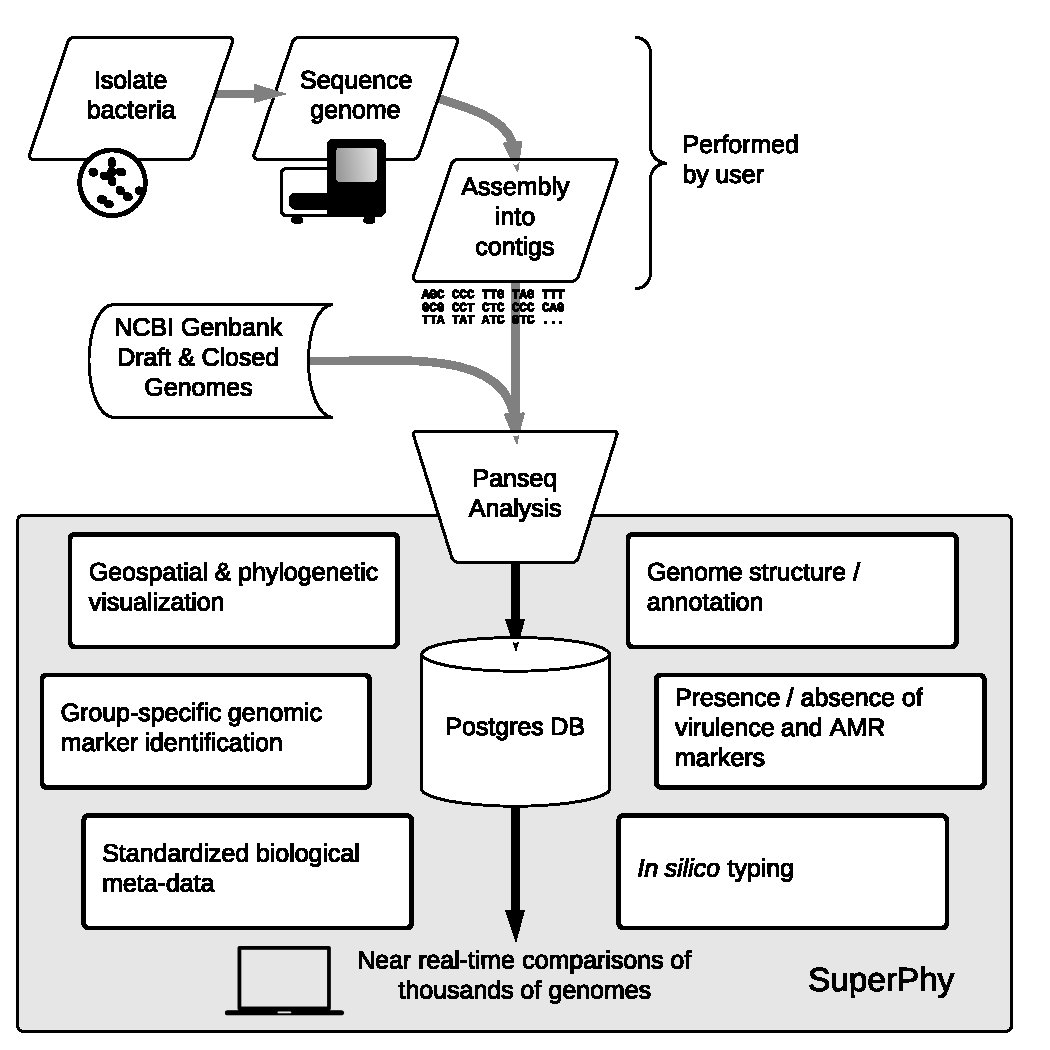
\includegraphics[width=13cm]{capabilities.pdf}}
  \caption{Overview of capabilities in the SuperPhy platform.}
  \label{fig:capabilities}
  %\vspace{-0.1cm}
\end{figure*}

The initial release of SuperPhy contains all publicly available data for \textit{Escherichia coli}, and includes expert-guided analyses of species-specific pathogroups and virulence determinants. In the future, SuperPhy will be expanded by the community to provide expert-guided analyses of additional species of bacterial pathogens for use by clinicians, epidemiologists and evolutionary biologists.

\section{\uppercase{Design}}
\label{sec:design}

\noindent SuperPhy is an interactive web platform that integrates public \textit{E. coli} genome data with genomic analyses tools. 1021 closed and draft E. coli genome sequences were downloaded from GenBank and incorporated into the SuperPhy database. Users can upload their own genome sequences for analysis to be kept private, or to be integrated into the public dataset. The platform is designed to be flexible and can work with closed genomes or genomic contigs from the assembly stage. 

\subsection{Database Schema}

The current focus of the SuperPhy platform is on analyzing \textit{E.coli}; however, SuperPhy was designed from the start to be extensible to other species. To make the database flexible, we chose to use the Chado relational schema \cite{mungall2007chado}. Chado was originally developed for storing model organism genomic data, but because of the central role of ontologies in Chado, it is also suited to storing genomic meta-data needed for phylogenetic and epidemiological analyses. In Chado, ontologies are used to assign types to entities, attributes and relationships \cite{mungall2007chado}. This ontology-centric design makes Chado highly adaptable. By not defining types in relational layers and instead using a mutable controlled vocabulary to assign types, the schema can be easily re-used or changed over time without having to change the relational structure \cite{mungall2007chado}.  Figure \ref{fig:ontology} shows the main entity types and corresponding relationship types used in our SuperPhy instance of the Chado schema (not shown are the attributes such as sequence locations or  meta-data). \texttt{Contig Collection} is the parent term assigned to any genome project uploaded by a user or obtained from an external database.  It does not directly contain any sequence data; it is used to store global attributes for a genome. A \texttt{Contig Collection} will be linked to one or more DNA sequences that are labeled \texttt{Contig}. The \texttt{Contig} types can be assembled contigs or fully closed chromosomes or plasmids (molecular type is distinguished at the attribute level). \texttt{Contig} and \texttt{Contig Collection} make up the supplied genome data. Further experimental features are calculated and added for each genome. The presence of Pan-genome loci in the individual isolate genomes is recorded using the \texttt{Locus} type. SNPs are calculated and recorded in the conserved core genome regions. Alleles of known virulence factors and antimicrobial resistance genes are identified and recorded with the allele type.  A more detailed description of the pipeline for identifying SNPs, loci and alleles is provided in section \ref{sec:pipeline}.

\begin{figure*}[t]
  \vspace{-0.2cm}
  \centering
   {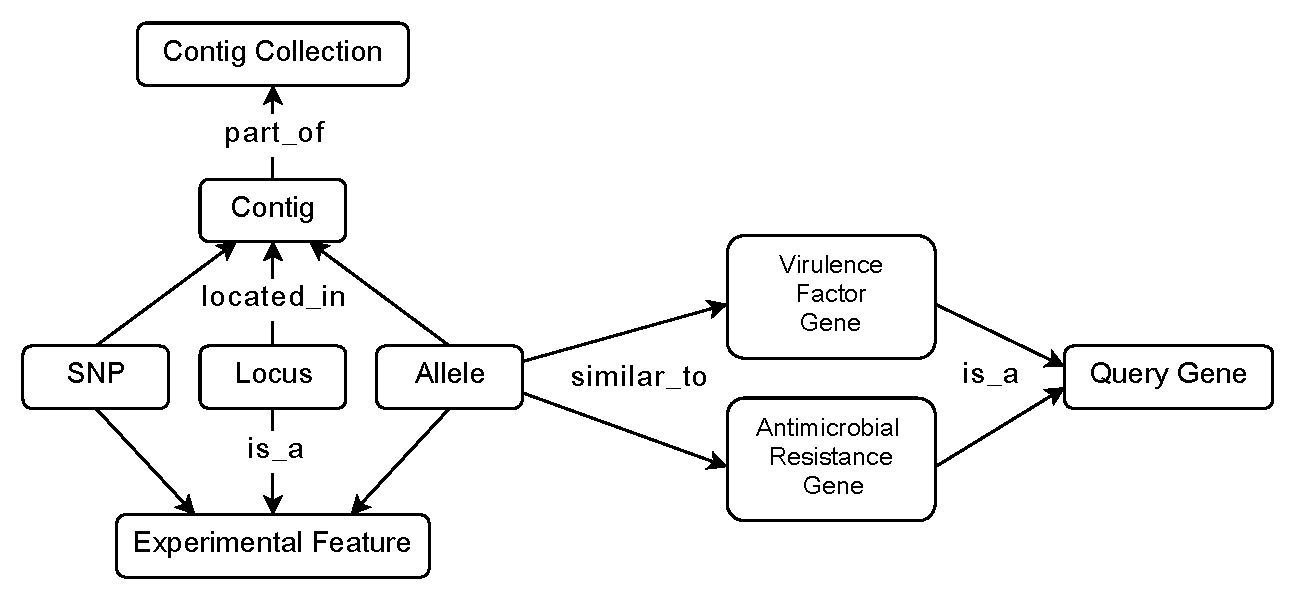
\epsfig{file = ontology.eps, width = 12cm}}
  \caption{A ontology graph representing the main feature types used in the SuperPhy schema.}
  \label{fig:ontology}
  %\vspace{-0.1cm}
\end{figure*}

\subsection{Analysis Pipeline}
\label{sec:pipeline}

Panseq is used as the computational engine for the SuperPhy platform \cite{laing_pan-genome_2010}. Genome sequences uploaded by users or obtained from NCBI GenBank Genome and Whole Genome Sequence repositories \cite{benson2013genbank} are input into Panseq to identify segments that belong to the conserved core genome and to the more variable accessory genome. Panseq works by iteratively aligning genomes using the MUMmer 3 program to produce a non-redundant pan-genome sequence \cite{laing_pan-genome_2010,kurtz2004versatile}. The pan-genome is then compared back to the input genomes to generate a listing of the presence or absence of each genomic locus in the pan-genome across the input genomes. Panseq also catalogs the SNP variations in the conserved regions \cite{laing_pan-genome_2010}.  The loci and SNPs identified by Panseq are loaded into the SuperPhy database. Annotations for the pan-genome regions are determined using a BLASTx analysis against the GenBank NR protein database.

A second analysis identifies virulence and antimicrobial drug resistance determinants in the genomes. Starting with a predefined set of query virulence factor (VF) and antimicrobial resistance (AMR) genes, the Panseq tool searches for alleles of these genes in the input genomes. Panseq uses BLASTn to conduct the search. The non-redundant query set of AMR genes was created by downloading the entire Comprehensive Antibiotic Resistance Database (CARD) \cite{mcarthur2012card} and subsequently clustering the CARD sequences based on similarity using BLASTclust \cite{altschul_gapped_1997}. Representatives from each cluster were selected first on the basis of the phylogenetic distance of the species to \textit{E. coli} and secondly, on the length where longer sequences were selected over shorter ones. All query AMR genes are organized according to their Antibiotic Resistance Ontology annotation to aid in identifying the presence of different antimicrobial resistance mechanisms \cite{antezana_biological_2009}. The VF gene set was produced by obtaining all gene alleles of known virulence factors in \textit{E. coli} from the Virluence Factor Database \cite{chen2012vfdb,chen2005vfdb}.  The longest allele was selected for each VF gene, except in cases where sequence similarity was less than 90\%, in which case, multiple alleles were included in the VF query set for a particular gene.

\subsubsection{Constructing and Displaying Phylogenetic Trees}

Global phylogenetic trees in SuperPhy are used in the results displays to show the phylogenetic position of a genome and also in the query forms, to allow users to select genomes based on tree location. A maximum-likelihood phylogenetic tree is constructed for all \textit{E. coli} genomes in the database using FastTree v2.1 \cite{price_fasttree_2010}. The tree is built from a multiple sequence alignment of the conserved core genome regions among all genomes, but is dynamically pruned based on user-selection to show specific genomes. The phylogenetic tree is displayed graphically using the D\sup{3} javascript library \cite{bostock2011d3}. The graphical interface was designed to be interactive; providing the ability to pan, zoom and expand, collapse or select tree nodes.

\subsubsection{Assigning Stx Subtypes}

The alleles for the A and B subunits from both \textit{stx1} and \textit{stx2} were collected in an analogous manner to the alleles for the virulence and AMR genes among all database strains, using as input the \textit{stx1} and \textit{stx2} subunit alleles from \textit{E. coli} strain O157:H7 Sakai ??need to check this??. A phylogenetic tree of all database strains based on each of \textit{stx1} and \textit{stx2} was created, and clades specific to a Shiga-toxin subtype were identified based on the scheme presented by Scheutz et al. (2012) \cite{scheutz_multicenter_2012}. Identification of Shiga-toxin subtype is therefore done through membership in pre-defined clades; those strains that fell outside of known sub-type clades are marked as unknown.

SuperPhy also allows the comparison of alleles among Shiga-toxin genes by displaying the multiple-sequence alignment for the user-selected strains. Users can then scroll through the alignment, where polymorphisms are highlighted for easy identification of differences.

\subsection{Meta-data}

Meta-data is invaluable in the biological interpretation of genome sequence data, but to maximize its usefulness, meta-data must be standardized. We developed in SuperPhy a predefined set of meta-data fields and permissible values. The meta-data types capture the key bacterial isolate attributes that characterize \textit{E. coli} infections. User compliance with these meta-data standards is aided by using context-dependent drop-down fields in the genome upload form. Selecting one of the fields will alter the available options in other fields (for example, selecting \textit{H. sapiens} as the host species will change the isolation sources and disease options that the user can select).  However, we also find it necessary to allow users to optionally define values for certain meta-data types such as the diseases and symptoms associated with an isolate. Table \ref{tab:metadata} shows the meta-data types employed in SuperPhy.

\begin{table*}[t!h]
\caption{Genome meta-data captured in the SuperPhy database. The meta-data values for genome O103:H25 Str. NIPH-11060424 are included as an example. N/A indicates the value was not defined or is not applicable to the SuperPhy genome project type.}
\label{tab:metadata} \centering
\begin{tabular}{|l|c|p{4.9cm}|p{5.6cm}|}
  \hline
  \textbf{Field} & \textbf{Required} & \textbf{Description} & \textbf{Example} \\
  \hline
  Name &  \checkmark & Genome name & O103:H25 Str. NIPH-11060424 \\
  \hline
  Host & \checkmark & Species that was source of isolate & Homo sapiens (human) \\
  \hline
  Source & \checkmark & Source tissue or material for isolate & Stool \\
  \hline
  Serotype & \checkmark & Antigen type designation & O103:H25 \\
  \hline
  Strain & \checkmark & Organism subtype & NIPH-11060424 \\
  \hline
  Date & \checkmark & Date isolate was obtained & 2006-01-01 \\
  \hline
  Molecular type & \checkmark & Chromosome, plasmid or contig & N/A \\
  \hline
  Genome type & \checkmark & Status of genome sequencing & WGS \\
  \hline
  Location &  & Location isolate was obtained from & Norway\\
  \hline
  Syndrome &  & Associated diseases or symptoms & Hemolytic-uremic syndrome \\
  \hline
  Age &  & Host age & N/A \\
  \hline
  PMID &  & Pubmed IDs of associated articles & PMID:22403614 \\
  \hline
  External ID &  & External DB accessions &   BioProject: 74417, genbank: AGSG00000000.1, taxon: 1101440 \\
  \hline
  Description &  & Genome description & Escherichia coli O103:H25 str. NIPH-11060424, whole genome shotgun sequencing project. \\
  \hline
  Comments &  & Free-form comments by submitter & The Escherichia coli O103:H25 str. NIPH-11060424 whole genome shotgun (WGS) project has the project accession AGSG00000000. This version of the project (01) has the accession number AGSG01000000, and consists of sequences AGSG01000001-AGSG01000491. Assembly Date :: NOV-2006 Assembly Method :: Newbler v. 1.0 Genome Coverage :: 20x Sequencing Technology :: Roche-454 \\
  \hline
  Keywords &  & Keywords to characterize genome & N/A \\
  \hline
  Closed &  & Indicates closed genome sequence & no \\
  \hline
  Owner &  & Source laboratory & Lindback,T., L'Abee-Lund,T.M. and Bohlin,J.. Submitted (14-OCT-2011) Dep of Food safety and Infection Biology, Norwegian School of Veterinary Science, Ullevalsveien 72, Oslo, Oslo 0033, Norway \\
  \hline
\end{tabular}
\end{table*}

\section{\uppercase{Functionality}}
\label{sec:functionality}

\subsection{Uploading a Genome}

Users can upload their \textit{E. coli} genomes to SuperPhy for analysis and comparison to the other \textit{E. coli} genomes in the database.  Access to uploaded genomes is regulated by the user. Users can select to keep their genome data private indefinitely, immediately make it publicly accessible, or choose to release it after a specified date, where it will automatically be added to the public data.  While private, users can grant other users access to their genomes.  Access is defined by three schemes: view only, modify (additionally allows users to change meta-data) and admin (provides full privileges to modify, delete or grant additional access to the genome).

\subsection{Retrieving Genome Meta-data}

Existing \textit{E. coli} genomes from the NCBI GenBank and Whole Genome Sequence repositories \cite{benson2013genbank} have been loaded into the SuperPhy database. Meta-data in these sources were mapped to our standardized set of meta-data types and values (see Table \ref{tab:metadata}). To facilitate navigation,
users can choose to display one or more of several types of meta-data in the forms (accession, serotype, strain, host species, isolation source, isolate date can be displayed alongside genome name). Through the advanced search facility, genome information can be queried by selecting from a interactive phylogenetic tree, from a world map, by date range or by boolean search of user-defined search fields and keywords.  The sophisticated query interface is designed to facilitate a broad range of hypotheses testing based on meta-data or phylogenetic information (Figure \ref{fig:search}).

\begin{figure*}[t]
  \vspace{-0.2cm}
  \centering
   {
\includegraphics[width=16cm]{superphy_forms.pdf}}
  \caption{Advanced search function in SuperPhy. Genome information can be queried by (A) interactive phylogenetic tree (B) world map or (C) boolean search of user-specified fields and keywords.}
  \label{fig:search}
  %\vspace{-0.1cm}
\end{figure*}

\subsection{Manipulating Geospatial Data}
SuperPhy presents a unique map tool, which uses Google Maps JavaScript API v3 (\url{https://developers.google.com/maps/documentation/javascript/}). It allows users to select \textit{E.coli} genomes obtained from various locations across the world. Users are initially presented with an overview of the world map along with a selectable list of all genomes in the SuperPhy database that have available location data. As users zoom in/out and/or pan across the map to a particular location, the list of selectable genomes changes to reflect those genomes in the current viewport of the map. This allows for users to refine the list of genomes on the map to a particular location of their choice. Users can additionally search for a location using the included search feature above the map. The map will automatically center on the location of interest and the selectable genome list will be updated to reflect any available genome sequence data from strains obtained within the area.  

\subsection{Groupwise Comparisons of the Distribution of SNPs and the Presence / Absence of Variable Genomic Loci}

The \textit{E. coli} pan-genome is highly variable, with approximately 80\% of an individual genome comprised of variable, accessory genes and only 20\% from the core-genome \cite{lukjancenko_comparison_2010}. To help correlate phenotype and genotype, SuperPhy provides the ability to compare between groups the presence or absence of pan-genome loci, as well as the distribution of SNPs within shared genome regions. A single consolidated pan-genome is computed from the individual genomes in the SuperPhy database. To identify group-specific or group-dominant genome regions or SNPs, the groupwise comparison function of SuperPhy allows users to select genomes in two comparison groups and returns the set of nucleotide variations or genome regions that are statistically enriched in one group compared to the other. The statistical enrichment is determined by the Fisher's Exact test as implemented in the R statistical language \cite{R_manual}.


\subsection{Identifying Virulence and Antimicrobial Drug Resistance Determinants}

SuperPhy provides analyses for identifying and evaluating risk factors. Users can examine the distribution of the presence or absence of virulence and AMR markers in the genomes.  Pre-defined sets of characterized virulence factors and antimicrobial resistance genes were collected and examined for their presence among all individual genomes \cite{mcarthur2012card,chen2012vfdb,chen2005vfdb}. Users can query multiple specific markers in targeted genomes. The sequences of identified VF and AMR gene alleles in the individual genomes are stored in the database, as are the multiple sequence alignments of the alleles present in each individual strain. This allows the sequence-comparison among user selected strains to be displayed in real-time. 

\section{\uppercase{Examples of Use Cases}}
\label{sec:cases}
\subsection{Time Critical Genomic Analyses}
Example: A clinician has just received a bacterial isolate from a patient with gastrointestinal illness and would like to know the risk to the patient (how severe and what sort of illness is associated with the strain), the risk to the community (have these bacteria been isolated from other patients; is this an outbreak?) and possible treatment or prevention options. In order for the information to be to useful, the bacterial isolate must be characterized as soon as possible. The genome sequence is determined in the hospital using a distributed sequencing platform such as the MiSeq or IonTorrent and uploaded to SuperPhy. The clinician is within minutes presented with a summary of the strain for known and present virulence or AMR determinants, any novel genomic regions with respect to the genomes already present in the database, the phylogenetic positioning of the new isolate and closely related strains, and their geographical distribution. This clinician also has the opportunity to add the new strain to the shared public database, where it will instantly be available to the community of SuperPhy users.

In the current genomics landscape, it is impossible to perform the above analyses in the time required to make effective decisions. Results of this sort are usually historical and of no immediate clinical value. The same analysis would require knowledge of a number of bioinformatics programs, a local collection of strains to run the comparison against, a collection of virulence and antimicrobial factors, and a means of identifying unique genomic elements.

The entire process would take days and the knowledge gained would not be immediately available to others. With our novel integration of the data and computational approaches, the analyses can be performed in minutes, a summary generated, and both the genome and
information about that genome stored and available for other users, saving duplication of analyses and increasing the value of the computational platform. The rate-limiting step for the platform is now the deposition of genome sequence data.

\subsection{Identification of Genomic Novelty Informing Phenotype}
Examples: 1) An epidemiologist has identified a pathogen responsible for high levels of severe illness and wishes to identify genomic regions that are present in the pathogen but absent among closely related strains not implicated in human disease; 2) An agricultural researcher wishes to identify genomic elements statistically associated with \textit{E. coli} strains that are shed from cattle more frequently and in higher amounts than other \textit{E. coli} found in the bovine gastrointestinal tract; 3) A researcher in the oil industry wishes to identify novel genes in a bacterial strain that has been shown to break down hydrocarbons at a rate greater than other bacteria; 4) An environmental scientist wishes to identify genomic regions that allow one group of bacteria from a species to persist in an environment that is toxic to other groups of bacteria of the same species.

As the SuperPhy computational tools are tightly coupled with the underlying data, all metadata (source, host, severity of illness, etc.) are immediately available for determining phenotypic groups that can be compared at the genomic level. Additionally, the spatial distribution of genomic sequences is displayed in map form, allowing the user to `zoom-in' and graphically select a region of interest. The presence / absence of all genomic regions and single-nucleotide polymorphisms among shared genomic regions is also pre-computed, enabling the identification of genomic regions that are statistically different between groups, be they based on severity of illness, host, or geographical location.

The results are then made available for download and the analysis saved in the platform for others to use with permission of the original user.

\subsection{Discovery Research}
Example: A genomics researcher has obtained the assembled contigs from an Illumina sequencing run, generating 200 novel genomic sequences in an underrepresented bacterial species responsible for infrequent but severe cases of human disease. He wishes to quickly identify the phylogenetic relationships among these bacteria and all previously sequenced genomes, as well as to identify virulence and AMR genes, and novel genomic regions present in the strains with respect to closely related genomic sequences. The researcher simply uploads his sequences to SuperPhy, after which the new strains are placed on the phylogenetic tree of all strains, and the presence of any known virulence / AMR genes is determined. Lastly, the 200 new strains are compared to the pre-computed genomics database, where any novel genomic regions are identified for the researcher.

\section{\uppercase{Collaboration and Community Benefit}}
\label{sec:collaboration}
There are currently similar projects underway world-wide with a similar goal: to provide a platform for comparative genomic epidemiology \cite{kupferschmidt_outbreak_2011}. The transfer of strains across international borders can be time consuming or impossible, whereas the exchange of genome sequence information can happen as soon as it becomes available. These international efforts with common goals should at the least provide data in a format that allows for it to be easily shared and understood among the various platforms. The value to the community of users of this shared computational resource increases as the number of users contributing data to it increases, which in turn makes the platform more attractive to use and contribute to by others.

\section{\uppercase{Availability}}
\label{sec:availability}

The website is available at http://lfz.corefacility.ca/superphy/. The software code and database will be made available upon request.

\section{\uppercase{Conclusions}}
\label{sec:conclusion}

\noindent SuperPhy is a broadly accessible, integrated platform for the phylogenetic and epidemiological analyses of bacterial genome data. It provides near-real time analyses of thousands of genomic sequences using novel computational approaches with results that are understandable and useful to a wide community, including those in the fields of clinical medicine, epidemiology, ecology and evolution. The web-interface to this computational platform obviates the need for command-line skills, or a particular computer environment. As additional members of the research community use the platform, the number of genomic sequences stored and analyzed will increase, adding further value to the platform, and in turn attracting more users. Genomic platforms such as SuperPhy will become increasingly important in transforming raw genomic data into a format suitable the development of a world-wide real-time surveillance and analyses network for bacterial genomes.

\section*{\uppercase{Acknowledgements}}

\noindent This work was funded by the Public Health Agency of Canada and a grant from the Canadian Genomics Research and Development Initiative. We would like to thank the following students for their work on this project: Omar Zabaneh, Michael Benediktson, Peter Shen and Waqar Gill. We would like to thank the Canadian Food Inspection Agency for allowing this work to be conducted at the Animal Diseases Research Institute.


\vfill
\bibliographystyle{apalike}
{\small
\bibliography{bioinformatics2014}}

\vfill
\end{document}
